\clearpage

\begin{nquote}{}
	``The shape of water -- woman falls in love with monster; fine. However, the shape of water is a beautiful phrase, because water has no shape!" - Dr. Loewen, 10/30/2023
	
	\medskip
	
	``Metric\dots is that Greek for measurement? Might be." - Dr. Loewen, 10/30/2023
	
	\medskip
	
	``Why are 320 lectures so slow? Well I've been teaching calculus for decade, I've had to slow down for the civilians." Dr. Loewen, 10/30/2023
\end{nquote}

\section{Point-set topology}

\subsection{Open sets}

\subsubsection*{Step 1: Euclidean \(\R^k\)}
Recall \(\R^k=\{(x_1,\dots,x_k):x_j\in\R\}\) with \(|\mvec{x}|=\sqrt{x_1^2+x_2^2+\dots+x_k^2}\).
\begin{ndef}{: Open set}
	A subset \(\mc{U}\subseteq\R^k\) is \emph{\textbf{open}} iff for all \(x\in\mc{U}\), there exists \(\eps>0\) such that for all \(x'\) with \(|x'-x|<\eps\), \(x'\in\mc{U}\).
\end{ndef}
The following diagram provides intuition:
\begin{figure}[htbp]
	\centering
	\begin{tikzpicture}
		\draw[thick, dotted, black, thick, fill = white!60!gray] (0, 0.6) to [curve through ={(1.8, 0.475)..(4.75, 0.4)..(4.8, 0.02)..(5, 0)..(4.9, -0.25)..(4.75, -0.76)..(2.5, -0.72)..(0, -1)..(-1.85, -0.78)..(-1.9, -0.4)..(-2, 0)..(-1, 0.5)}] (0, 0.6);
		\node[above] at (-1.5, -0.3) {\(\mc{U}\)};
		\draw[thick, dotted, black, fill = gray!60!lightgray] (3.7, 0.3) circle (20pt);
		\node[below] at (3.7, -0.35) {\(\B[x;\eps)\)};
		\draw[fill] (3.7, 0.3) circle (1pt);
		\node[below] at (3.7, 0.3) {\(x\)};
		\draw[<->] (3.7, 0.32) -- (3.7, 1);
		\node[right] at (3.7, 0.64) {\(\eps\)};
	\end{tikzpicture}
	\caption{Visualization of an open set.}
\end{figure}

\begin{note}
	Call \(\B[x;\eps)\) with \(\eps>0\) an ``open ball with centre \(x\) and radius \(\eps\)." It does indeed deserve to be called open: pick some \(y\in\B[x;\eps)\); thus \(r=|y-x|<\eps\). Here, \(\eps-r>0\), and \(\B[y;\eps-r)\subseteq \B[x;\eps)\). To verify, pick some \(z\in\B[y;\eps-r)\). Then
	\begin{align*}
		|z-x|\leq&|z-y|+|y-x|\\
			    <&(\eps-r)+r=\eps.
	\end{align*}
	
	The following diagram provides intuition:
	\begin{figure}[htbp]
		\centering
		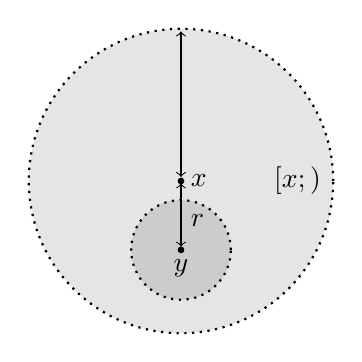
\begin{tikzpicture}
			\draw[dotted, thick, fill = white!60!lightgray] (0, 0) circle (55pt);
			\draw[fill] (0, 0) circle (1pt);
			\node[right] at (0, 0) {\(x\)};
			\node[right] at (0, 0.95) {\(\eps\)};
			\draw[<->] (0, 0.05) -- (0, 1.9);
			\node[left] at (1.9, 0) {\(\B[x;\eps)\)};
			\draw[dotted, thick, fill = white!60!gray] (0, -0.875) circle (18pt);
			\draw[fill] (0, -0.875) circle (1pt);
			\node[below] at (0, -0.875) {\(y\)};
			\draw[<->] (0,-0.835) -- (0, -0.03);
			\node[right] at (0, -0.5) {\(r\)};
			%\draw[fill] (-0.25, -0.6) circle (1pt);
			%\node[right] at (-0.25, -0.6) {$x$};
			%\draw[] (-2.5, -2.5) -- (-2.5, 2.5) -- (2.5, 2.5) -- (2.5, -2.5) -- (-2.5, -2.5);
			%\node[right] at (2.5, -2.35) {\(\B[x;\eps)\)};
		\end{tikzpicture}
		\caption{Visualization of an open ball.}
		%\label{fig7}
	\end{figure}
\end{note}

\begin{notation}
	We define:
	\begin{enumerate}[(a)]
		\item An open ball as
		\begin{equation*}
			\B[x;\eps):=\{x'\in\R^k:|x'-x|<\eps\}.
		\end{equation*}
		
		\item A closed ball as
		\begin{equation*}
			\B[x;\eps]:=\{x'\in\R^k:|x'-x|\leq\eps\}.
		\end{equation*}
		
		\item A punctured ball as
		\begin{equation*}
			\B(x;\eps):=\{x'\in\R^k:0<|x'-x|<\eps\}.
		\end{equation*}
	\end{enumerate}
\end{notation}
\begin{ndef}{: Topology}
	We call \(\ms{T}\) a \emph{\textbf{topology}}, where
	\begin{equation*}
		\ms{T}:=\{\mc{U}\subseteq\R^k:\mc{U}~\text{is open}\}.
	\end{equation*}
	Here, \(\ms{T}\subseteq\ms{P}(\R^k)\).
\end{ndef}


There are a few key properties of \(\ms{T}\):
\begin{enumerate}[(HTS~1)]
	\item \(\emptyset\in\ms{T}\) and \(\R^k\in\ms{T}\).
	
	\item For \emph{any} collection \(\ms{G}\) of open sets, 
	\begin{equation*}
		\bigcup\ms{G}=\bigcup_{\mc{G}\in\ms{G}}\mc{G}
	\end{equation*}
	is also open.
	
	\item For any \emph{finite} collection of open sets \(\mc{G}_1,\dots,\mc{G}_N\), the set 
	\begin{equation*}
		\bigcap_{k=1}^N \mc{G}_k=\mc{G}_1\cap \mc{G}_2\cap\dots\cap \mc{G}_N
	\end{equation*}
	is also open.
	\begin{proof}
		Pick \(x\in\displaystyle\bigcap_{k=1}^N \mc{G}_k\). For each \(k\), \(x\in \mc{G}_k\implies\) there exists \(\eps_k>0\) such that \(\B[x;\eps_k)\subseteq \mc{G}_k\). Now, set \(\eps=\operatorname{min}\{\eps_1,\eps_2,\dots,\eps_N\}\) to see that \(\B[x;\eps)\subseteq \mc{G}_k\) for \emph{all} \(k\). Therefore, \(\B[x;\eps)\subseteq\displaystyle\bigcap_{k=1}^N \mc{G}_k\) .
	\end{proof}
	
	\item For any \(x,y\in\R^k\) -- where \(x\neq y\) -- there exists \(\mc{U},\mc{V}\in\ms{T}\) such that \(x\in\mc{U}\), \(y\in\mc{V}\), \(\mc{U}\cap\mc{V}=\emptyset\).
	\begin{proof}
		Let \(r=|x-y|>0\) and take \(\mc{U}=\B[x;r/3),~\mc{V}=\B[y;r/3)\). Picking some \(z\in\mc{U}\cap\mc{V}\) is an immediate contradiction:
		\begin{equation*}
			r=|x-y|\leq |x-z|+|z-y|<\frac{r}{3}+\frac{r}{3}.
		\end{equation*}
		
		The following diagram provides intuition:
		\begin{figure}[H]
			\centering
			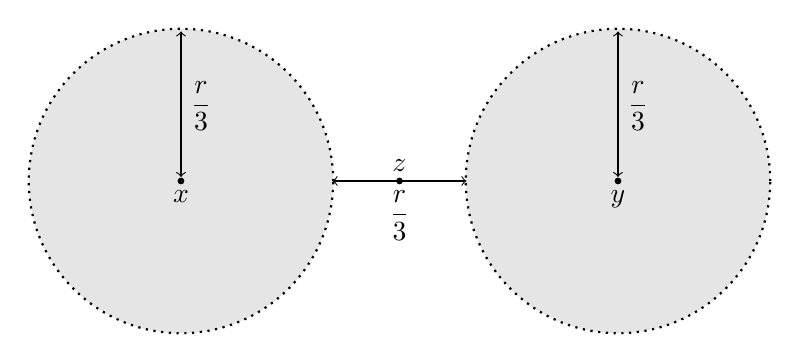
\begin{tikzpicture}
				\draw[dotted, thick, fill = white!60!lightgray] (-2.775, 0) circle (55pt);
				\draw[<->] (-2.775, 0.05) -- (-2.775, 1.9);
				\node[right] at (-2.775, 0.95) {\(\displaystyle\frac{r}{3}\)};
				\draw[dotted, thick, fill = white!60!lightgray] (2.775, 0) circle (55pt);
				\draw[fill] (-2.775,0) circle (1pt);
				\node[below] at (-2.775,0) {\(x\)};
				\draw[<->] (2.775, 0.05) -- (2.775, 1.9);
				\node[right] at (2.775, 0.95) {\(\displaystyle\frac{r}{3}\)};
				\draw[<-] (-0.85, 0) -- (0.025, 0);
				\draw[->] (0.025, 0) -- (0.85, 0);
				\draw[fill] (2.775,0) circle (1pt);
				\node[below] at (2.775,0) {\(y\)};
				\draw[fill] (0,0) circle (1pt);
				\node[below] at (0,0) {\(\displaystyle\frac{r}{3}\)};
				\node[above] at (0,0) {\(z\)};
			\end{tikzpicture}
			\caption{Visualization of HTS 4.}
			%\label{fig7}
		\end{figure}
	\end{proof}
\end{enumerate}
\begin{comment}
	\draw[dotted, thick, fill = white!60!gray] (0, -0.875) circle (18pt);
	\draw[fill] (0, -0.875) circle (1pt);
	\node[below] at (0, -0.875) {\(y\)};
	\draw[<->] (0,-0.835) -- (0, -0.03);
	\node[right] at (0, -0.5) {\(r\)};
	\draw[fill] (-0.25, -0.6) circle (1pt);
	\node[right] at (-0.25, -0.6) {$x$};
	\draw[] (-2.5, -2.5) -- (-2.5, 2.5) -- (2.5, 2.5) -- (2.5, -2.5) -- (-2.5, -2.5);
	\node[right] at (2.5, -2.35) {\(\B[x;\eps)\)};
\end{comment}
\begin{note}
	HTS stands for \emph{Hausdorff Topological Space}. The condition for a topological space for being Hausdorff is just (HTS 4); rest are true for general topological spaces.
\end{note}

\subsubsection*{Step 2: Metric spaces}
\begin{ndef}{: Metric}
	Given any set \(\mc{X}\neq\emptyset\), a function \(d:\mc{X}\times\mc{X}\to\R\) is called a \emph{\textbf{
	metric}} exactly when 
	\begin{enumerate}[(a)]
		\item \(d(x,y)\geq 0\) for all \(x,y\in\mc{X}\) with
		\begin{equation*}
			d(x,y)=0\iff x=y.
		\end{equation*}
		
		\item \(d(x,y)=d(y,x)\) for all \(x,y\in\mc{X}\)\qquad (Symmetry).
		
		\item \(d(x,z)\leq d(x,y)+d(y,z)\) for all \(x,y,z\in\mc{X}\)\qquad (Triangle inequality).
	\end{enumerate}
\end{ndef}
\begin{example}
	The following are examples are metrics:
	\begin{enumerate}[(a)]
		\item Euclidean \(\R^k\) has \(d(x,y)=|y-x|\); this is called the ``Euclidean metric".
		
		\item Recall
		\begin{equation*}
			\ell^2=\left\{x=(x_1,x_2,\dots)\st\sum_{k=1}^{\infty}x_k^2<\infty\right\}
		\end{equation*}
		with \(\norm{y-x}=\left[\displaystyle\sum_{k=1}^{\infty}(y_k-x_k)^2\right]^{1/2}=d(x,y)\) (we proved this in homework 7 problem 3.)
		
		\item For the set \(\mc{X}\) of bounded functions, \(f:[0,1]\to\R\), \(d(x,y)=\sup\{|x(t)-y(t)|\}\) works (we proved this in homework 5 problem 8.)
		
		\item For any \(\mc{X}\neq\emptyset\), take 
		\begin{equation*}
			d(x,y)=\begin{cases}
					0,&\text{if}~x=y\\
					1,&\text{if}~x\neq y
				   \end{cases}.
		\end{equation*}
		This is called the ``discrete metric".
	\end{enumerate} 
	\begin{reflection}
		Why do we care about all this anyways? The main reason -- at the moment at least -- is to extend the idea of \emph{convergence} to cover many structures at once.
	\end{reflection}
\end{example}